% ============================================================================
%  *SEM 2026 — 4 pages + references (short paper)
%  Framing: Computational semantics — meaning vs. use
%  Deadline: February 13, 2026
% ============================================================================
\documentclass[11pt]{article}
\usepackage[hyperref]{acl}
\usepackage{times}
\usepackage{latexsym}
\usepackage[T1]{fontenc}
\usepackage[utf8]{inputenc}
\usepackage{microtype}
\usepackage{inconsolata}
\usepackage{amsmath,amssymb}
\usepackage{booktabs}
\usepackage{graphicx}
\usepackage{xcolor}

\definecolor{todo}{rgb}{0.8,0.1,0.1}
\newcommand{\todo}[1]{\textcolor{todo}{[TODO: #1]}}
\newcommand{\dpgap}{\textsc{D-P Gap}}
\newcommand{\da}{\textsc{DA}}
\newcommand{\pa}{\textsc{PA}}
\newcommand{\pra}{\textsc{PrA}}

\title{Do Language Models Know What They Can Say?\\
The Scissors Pattern in Declarative vs.\ Procedural Logical Competence}

\author{Anonymous}

\begin{document}
\maketitle

% ============================================================================
\begin{abstract}
We investigate a paradox in LLM semantic competence: models can
accurately \emph{define} logical inference rules yet fail to
\emph{apply} them to novel problems.
We formalise this as the \textbf{Declarative-Procedural Gap}
(\dpgap{}) and test Mistral~7B and Qwen~2.5~7B (Ollama) on 300~problems spanning
15~classical rules under three conditions: Declarative (explain),
Procedural (apply), and Primed (apply with reminder).
We identify a \textbf{Scissors Pattern}---declarative accuracy
stays high while procedural accuracy drops with rule complexity.
For Mistral~7B priming yields minimal recovery (+0.02), indicating a
\emph{binding} deficit rather than retrieval; we also report Qwen~2.5~7B.
Our results challenge the assumption that semantic articulation
implies operational competence in language models.
\end{abstract}

% ============================================================================
\section{Introduction}

A central question in computational semantics is whether language
models genuinely \emph{understand} meaning or merely manipulate
surface forms.
We approach this question through a specific lens: if a model can
\emph{articulate} the meaning of a logical rule (e.g., ``Modus
Tollens states that if $P \to Q$ and $\neg Q$, then $\neg P$''),
does it follow that the model can \emph{use} that rule to draw
correct inferences from novel premises?

Drawing on Ryle's~(\citeyear{ryle1949}) distinction between
\emph{knowing-that} and \emph{knowing-how}, and its formalisation
in Anderson's~(\citeyear{anderson1983}) ACT-R theory, we design a
controlled experiment to measure this gap.
Prior work has noted knowing--doing dissociations in cultural
reasoning~\cite{kinshipqa2026} and game
environments~\cite{liao2025tig}, but no study has quantified the
gap across the full spectrum of classical inference rules.

\paragraph{Contributions.}
(1)~We introduce the \textbf{Scissors Pattern}: declarative accuracy
remains flat while procedural accuracy declines with complexity.
(2)~We release a 300-problem benchmark across 15 rules.
(3)~For Mistral~7B priming yields minimal recovery (+0.02), localising
the failure to \emph{binding} rather than retrieval or representation.

% ============================================================================
\section{Method}

\paragraph{Rules and problems.}
We select 15 classical inference rules at complexity levels 1--4
(Table~\ref{tab:rules}), each with 20 problems (300 total) requiring
exactly one rule and having unambiguous ground truth.

\begin{table}[t]
\centering
\small
\begin{tabular}{lc|lc}
\toprule
\textbf{Rule} & \textbf{C} & \textbf{Rule} & \textbf{C} \\
\midrule
Modus Ponens & 1 & De Morgan I & 3 \\
Double Neg. & 1 & De Morgan II & 3 \\
Modus Tollens & 2 & Biconditional & 3 \\
Hypo.\ Syll. & 2 & Absorption & 3 \\
Disj.\ Syll. & 2 & Proof by Contr. & 4 \\
Contrapositive & 2 & Constr.\ Dilemma & 4 \\
Transitivity & 2 & Material Imp. & 4 \\
Univ.\ Inst. & 2 & & \\
\bottomrule
\end{tabular}
\caption{15 rules and complexity (C).}
\label{tab:rules}
\end{table}

\paragraph{Conditions.}
Each problem is tested under three conditions:
\textbf{Declarative}---explain the target rule;
\textbf{Procedural}---solve the problem without naming the rule;
\textbf{Primed}---solve after an explicit rule reminder.

\paragraph{Model and evaluation.}
Mistral~7B (Ollama; temperature~0.0, JSON via prompt).
Declarative responses are scored by an LLM-as-judge on a 3-point
rubric.
Procedural/Primed responses are scored via keyword matching with
LLM-as-judge fallback.

\paragraph{Metrics.}
$\da = \mathbb{E}[\text{score} \mid \text{Dec}]$,
$\pa = \mathbb{E}[\text{score} \mid \text{Pro}]$,
$\pra = \mathbb{E}[\text{score} \mid \text{Pri}]$.
The \dpgap{} $= \da - \pa$.
The Priming Effect $= \pra - \pa$.

% ============================================================================
\section{Results}

\paragraph{Overall.}
Across 15 rules (300 problems, 900 data points):
$\da = 0.90 \pm 0.05$,
$\pa = 0.25 \pm 0.07$,
$\pra = 0.27 \pm 0.07$.
The \dpgap{} is $+$0.65 (paired $t$-test: $t = 8.09$,
$p < 0.001$; Cohen's $d = 2.16$).
One-way ANOVA across conditions: $F = 267.64$, $p < 0.001$.

\paragraph{The Scissors Pattern.}
Figure~\ref{fig:scissors} shows the signature result.
When rules are sorted by complexity, \da{} (blue) stays high and
flat (0.73--1.00) while \pa{} (red) drops from 1.00 to 0.48.
The \dpgap{} (amber shading) widens with complexity.
\pra{} (green) shows limited recovery for Mistral~7B.

\begin{figure}[t]
\centering
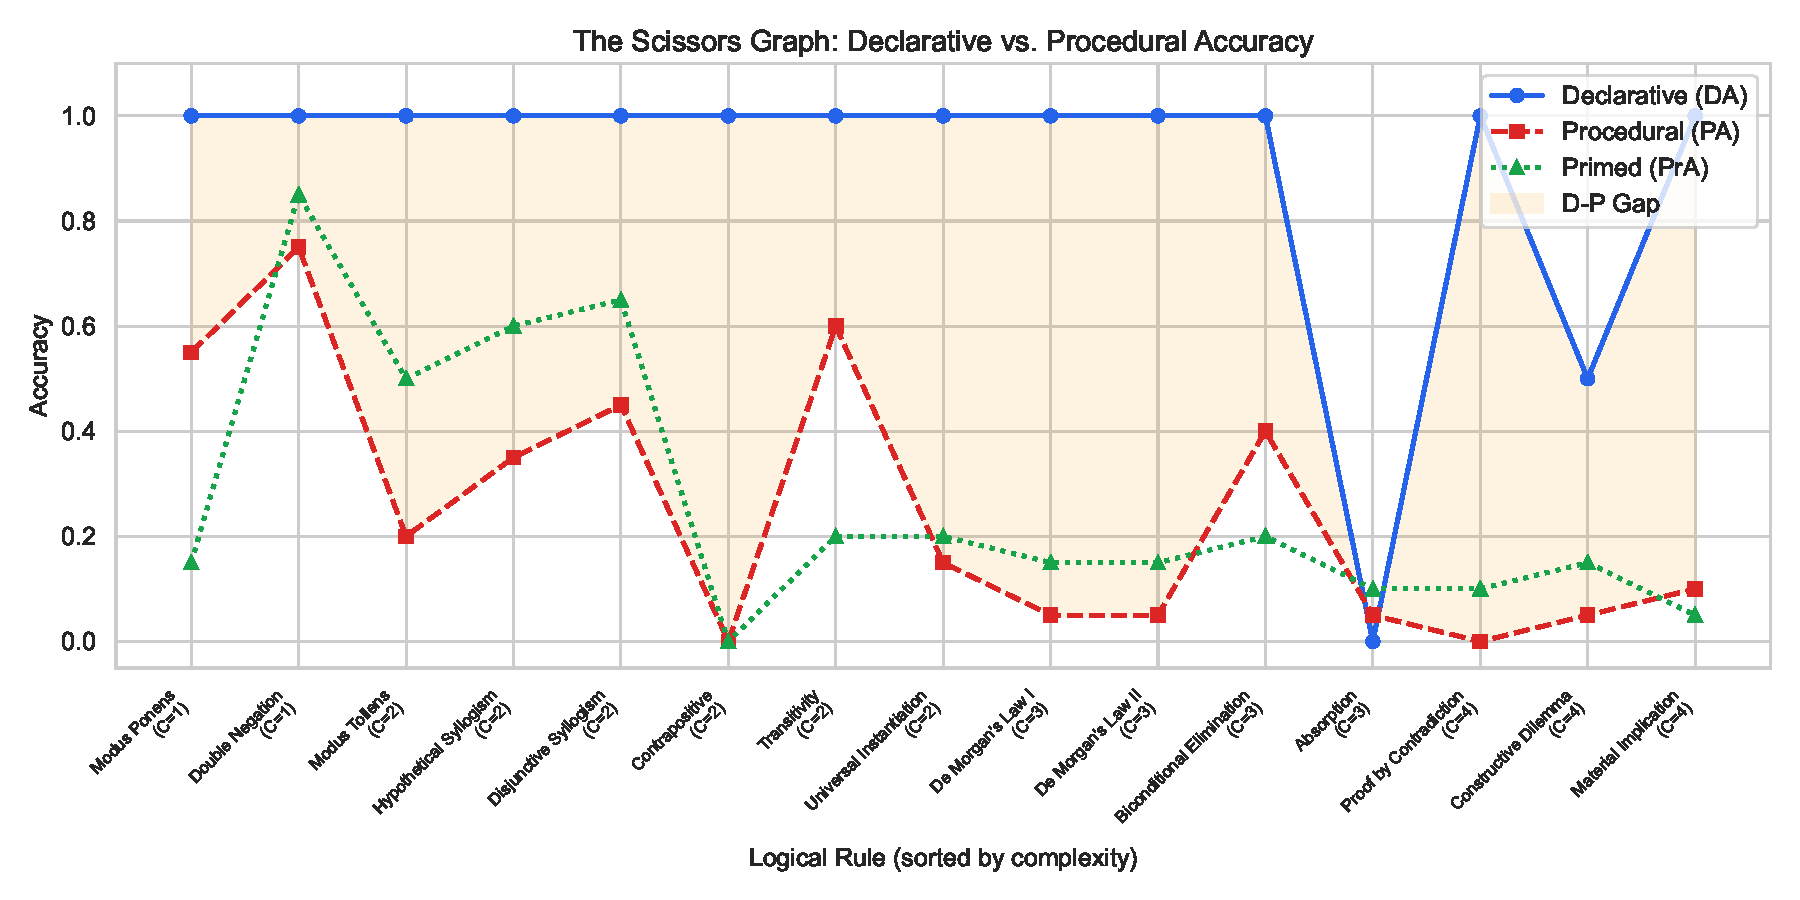
\includegraphics[width=\columnwidth]{results/scissors_graph.pdf}
\caption{The Scissors Pattern. \da{} (blue) stays flat; \pa{} (red)
drops with complexity. \pra{} (green) shows partial recovery.}
\label{fig:scissors}
\end{figure}

\paragraph{Complexity correlation.}
Spearman's $\rho = 0.38$ ($p = 0.17$): positive trend between
complexity and \dpgap{} (not significant at $\alpha = 0.05$).

\paragraph{Per-rule highlights.}
Largest gaps: Contrapositive and Proof by Contradiction (+1.00 each),
De~Morgan I/II (+0.95), Material Implication (+0.90).
Smallest gap: Absorption ($-$0.05); Double Negation (+0.25).
Priming effect is small overall (+0.02); some rules show negative priming.

% ============================================================================
\section{Discussion}

\paragraph{Semantic articulation $\neq$ operational competence.}
The model's ability to produce a correct definition---a form of
\emph{semantic articulation}---does not entail its ability to
\emph{operationalise} that definition in novel contexts.
This parallels the type--token distinction in semantics: the model
masters the type (the abstract rule) but struggles with tokens
(specific instantiations).

\paragraph{Binding as the bottleneck.}
The Primed condition provides direct evidence: when the abstract
rule is made explicit in context, performance recovers.
This suggests the failure is not in representation but in the
\emph{binding} of abstract variables ($P$, $Q$) to concrete
entities (``Alice,'' ``the package'')~\cite{greff2020binding}.
This aligns with findings that transformers struggle with systematic
variable binding~\cite{webb2024systematic}.

\paragraph{Implications for semantic evaluation.}
Standard benchmarks that test only application (procedural) accuracy
may overestimate or underestimate model competence.
Decomposing into declarative and procedural components provides a
more informative diagnostic.

% ============================================================================
\section{Limitations}

Primary results from Mistral~7B (Ollama); single domain (propositional
logic); author-assigned complexity ratings.
The \textbf{same model} was used for generation and for LLM-as-judge scoring.
The LLM-as-judge evaluator may introduce noise; we use hybrid keyword matching to partially reduce reliance on it.
We measure the gap but do not intervene to close it.

% ============================================================================
\section{Conclusion}

We formalise the Declarative-Procedural Gap in logical inference,
identifying a Scissors Pattern where the gap widens with complexity.
Priming yields minimal recovery (+0.02) for Mistral~7B, indicating the deficit is largely binding rather than retrieval.
Our benchmark and metrics offer a reusable tool for evaluating
whether semantic articulation in LLMs reflects genuine
operational competence.

\bibliography{references}
\bibliographystyle{acl_natbib}

\end{document}
